% Context, isothermal, thermodynamical framework, standard generalized material etc.
In this section, the mathematical laws allowing the description of the deformation of a solid body will be derived. First, the kinematic laws governing the motion of each material point belonging to a solid will be considered. The variations of lengths and shapes of a continuum, described by the \textit{strain} mesure will then be associated to internal forces through thermodynamic framework. Finally, the theory of first order quasi-linear partial differential system will be applied to solid dynamics in order to deliver analytical solutions for specific problems. The literature on the subject being very rich (see for instance \cite[Chapters~1-3]{Foundation_of_elasticity}, \cite{Truesdell}, \cite[Chapter~7]{Simo}, \cite[Chapters~3 \& 5]{Belytschko}), the governing equations of mechanics will be developed non-exhaustively.

\subsection{Kinematic laws -- Strain mesures}
We consider a three-dimensional solid domain with volume denoted by $\Omega \subset \Rbb^3$ bounded by the surface $\partial \Omega$. This body undergoes external sollicitations that can either be localized on a part of the external surface of the body (\textit{i.e. surface forces}) or act in the whole solid domain (\textit{i.e. volume forces}). Due to the presence of such sollicitations, the volume may change during a deformation within the time interval $\tau = \[0,T\]$ and will hence be written as a function of time $\Omega(t)$ ($t\in \tau$). The state of the solid at time $t=0$, corresponding to a non-deformed state with volume $\Omega(t=0)=\Omega_0$, is referred to as the \textit{initial configuration}. Some problems require the use of a \textit{reference configuration} that can be deformed and to which equations are referred. In what follows, the reference and initial conditions are identical. At a given time $t>0$, the volume $\Omega(t)=\Omega_t$ corresponds to the \textit{current configuration}. These configurations are depicted in figure \ref{fig:deformationFunction}.
\begin{figure}[h]
  \centering
  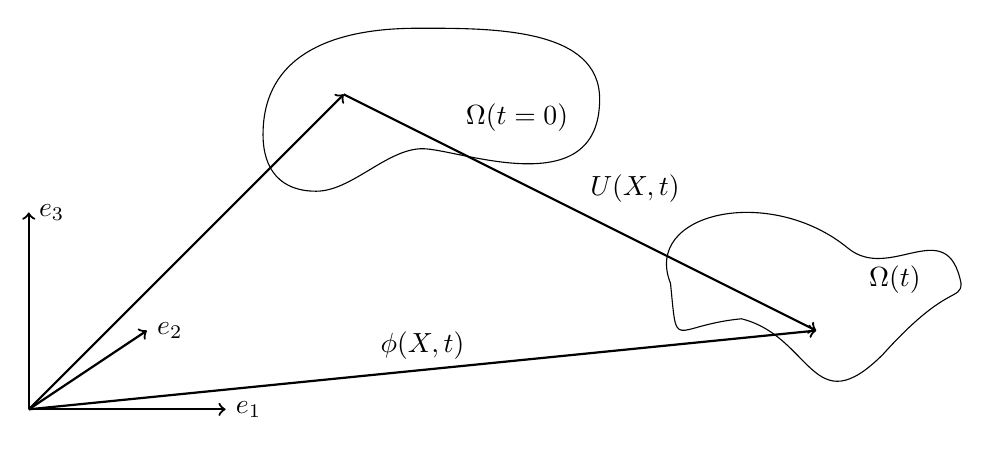
\begin{tikzpicture}
  %\draw[step=1.0,black,thin] (-3.,-1.) grid (3,4.);
  %\draw (-3,-1) -- (3,-1) -- (3,4) -- (-3,4) -- (-3,-1);
  \draw[thick,->] (-5,-2.5) -- (-2.5,-2.5) node [right] {$\vect{e}_1$};
  \draw[thick,->] (-5,-2.5) -- (-5,0.) node [right] {$\vect{e}_3$};
  \draw[thick,->] (-5,-2.5) -- (-3.5,-1.5) node [right] {$\vect{e}_2$};
  \begin{scope}[scale=0.45]
    \draw (-3,0.6) .. controls +(1,0) and +(-1,0) .. (0,1.8)  
    .. controls +(1,0) and +(0,-3) .. (5,3.2) 
    .. controls +(0,2) and +(2,0)  .. (0,5.2) 
    .. controls +(-1,0) and +(0,3) .. (-4.5,2.2) 
    .. controls +(0,-1) and +(-1,0).. (-3,0.6) ;
  \end{scope}
  \node at (1.2,1.2) {$\Omega(t=0)$};
  %% Deformed body +2.
  \begin{scope}[scale=0.9]
    \draw (0.+0.5+4.,0-1.5) ..controls (1.+0.5+4.,-0.25-1.5) and (1.+0.5+4.,-1.5-1.5) .. (2.+0.5+4.,-0.5-1.5) ..controls (2.9+0.5+4.,0.5-1.5) and (3.1+0.5+4.,0.25-1.5) .. (3.1+0.5+4.,0.5-1.5) ..controls (2.9+0.5+4.,1.5-1.5) and (2.1+0.5+4.,.5-1.5) .. (1.5+0.5+4.,1.-1.5) ..controls (0.4+0.5+4.,1.9-1.5) and (-1.4+0.5+4.,1.5-1.5) .. (-1.+0.5+4.,0.5-1.5)..controls (-0.4+0.+4.,-0.-2.) and (-1+0.5+4.,0.4-2.) .. (0+0.5+4.,0-1.5);
  \end{scope}
  \node at (6.,-0.85) {$\Omega(t)$};
  \draw[->,thick] (-5,-2.5) -- (-1.,1.5) node [midway,left] {$\X$};
  \draw[->,thick] (-5,-2.5) -- (5.,-1.5) node [midway,above] {$\vect{\phi}(\vect{X},t)$};
  \draw[->,thick] (-1.,1.5) -- (5.,-1.5) node [midway,above right] {$\vect{U}(\vect{X},t)$};
\end{tikzpicture}

%%% Local Variables:
%%% mode: latex
%%% TeX-master: "../../mainManuscript"
%%% End:
  \caption{Deformation of a solid body between a reference state $\Omega_0$ to a subsequent state $\Omega_t$.}
  \label{fig:deformationFunction}
\end{figure}

In the reference configuration, every material particle is located by their position vectors: $\vect{X}=X_\alpha \vect{e}_\alpha$, where $X_\alpha$ denotes the \textit{Lagrangian coordinates} and $\vect{e}_\alpha$ the basis vectors. At a subsequent time $t$, the particle initially located at $\vect{X}$ may have moved and its current location is given by the smooth mapping $\vect{\phi}(\vect{X},t)=\phi_i(\vect{X},t)\vect{e}_i$. Thus, the mapping $\vect{\phi}$ provides the paths of every particle of the solid during the deformation. In the Lagrangian coordinates system, every particles are tracked during the deformation while the \textit{Eulerian coordinates}, denoted by $\vect{x}=x_i\vect{e}_i$, correspond to a \textit{spatial description}.
Note that in the above definitions Greek indices are used for quantities evaluated in the reference configuration whereas Latin ones refer to quantities defined in the current configuration. 

The \textit{displacement} and \textit{velocity} vectors of a particle between the reference and the current configuration are respectively:
\begin{subequations}
  \begin{alignat}{2}
    &\vect{u}(\vect{X},t)=\vect{\phi}(\vect{X},t) - \vect{X} \qquad \forall\:\: \vect{X},t \in \Omega_0\times \tau  \label{eq:displacement}\\
    &\vect{v}(\vect{X},t)=\drond{\vect{\phi}}{t}(\vect{X},t) = \vect{\dot{\phi}}(\vect{X},t) \qquad  \forall\: \: \vect{X},t \in \Omega_0\times \tau  \label{eq:velocity}
  \end{alignat}
\end{subequations}
where the superposed dot denotes the material time derivative. Furthermore, the second-order two-point \textit{deformation gradient} tensor is defined as:
\begin{equation}
  F_{i\alpha}=\drond{\phi_i}{X_{\alpha}}(\vect{X},t)  \label{eq:F_phi}
\end{equation}
or, by using equation \eqref{eq:displacement}:
\begin{equation}
  F_{i\alpha}= \drond{u_i}{X_\alpha} + \delta_{i\alpha} \label{eq:F_displacement}
\end{equation}
where $\delta_{i\alpha}$ is the \textit{Kronecker} symbol. The deformation gradient tensor characterizes the variations of lengths, areas and volumes. Indeed, the infinitesimal vector, oriented surface and volume elements respectively denoted by $\vect{dX},\vect{dS}$ and $dV$ and defined in the reference configuration transorm respectively to:
\begin{equation}
  \label{eq:transport_equations}
  \begin{aligned}
    & dx_i=F_{i\alpha}dX_\alpha \\
    & ds_i=J F_{\alpha i}^{-1}dS_{\alpha} \\
    & dv=JdV 
  \end{aligned}
\end{equation}
in the current configuration. The transport equations \eqref{eq:transport_equations} involve the determinant of the deformation gradient $J=\det(\tens{F})>0$, also called the \textit{Jacobian of the deformation}. The deformation gradient is a strain mesure since it accounts for changes in lengths and angles (\textit{i.e. the change of shape of a body}). Other strain mesures can be used as the \textit{right Cauchy-Green} or the \textit{Green-Lagrange} tensors, respectively defined as:
\begin{equation*}
  \begin{aligned}
    & \tens{C}=\tens{F}^T\tens{F} \\
    & \tens{E}=\frac{1}{2}(\tens{C}-\tens{I})
  \end{aligned}
\end{equation*}
where $\tens{I}$ is the second-order identity tensor. The Green-Lagrange tensor can also be written by means of equation \eqref{eq:F_displacement}:
\begin{equation*}
  \tens{E}=\frac{1}{2}(\drond{\vect{u}}{\vect{X}} + \drond{\vect{u}}{\vect{X}}^T + \drond{\vect{u}}{\vect{X}}\drond{\vect{u}}{\vect{X}}^T)
\end{equation*}
In particular, when the deformation involves displacement vectors such that $\norm{\drond{\vect{u}}{\vect{X}}} \ll 1$, the last (second-order) term of the previous definition can be neglected leading to:
\begin{equation*}
  \tens{E} \approx \frac{1}{2}(\drond{\vect{u}}{\vect{X}} + \drond{\vect{u}}{\vect{X}}^T) = \tens{\eps}
\end{equation*}
with $\tens{\eps}$ the \textit{linearized strain tensor}, the symmetric part of the displacement gradient. Such deformations fall in the \textit{linearized geometrical framework} and are characterized by small strain but possibly large displacements. Furthermore, when the deformation leads to a displacement vector $\norm{\vect{u}} \ll 1$ reference and current configurations are considered as indentical. These situations correspond to the \textit{small strain} framework. 

\subsection{Balance equations}
Recall that these works relate to the numerical simulation of solid mechanics problems with a material descritption of the motion. Thus, we will now focus on Lagrangian local balance laws. The \textit{linear momentum} is defined as $\vect{p}(\vect{X},t)=\rho(\vect{X},t)\vect{v}(\vect{X},t)$ and satifies during a deformation \cite[Chapter~2]{Truesdell}:
\begin{equation}
  \label{eq:Lagrangian_linear_momentum}
  \rho_0(\vect{X}) \vect{\dot{v}}(\vect{X},t) - \nablav_0 \cdot \tens{\Pi}(\vect{X},t) = \rho_0(\vect{X}) \vect{b}(\vect{X},t) \qquad \forall \: \: \vect{X},t \in \Omega_0 \times \tau 
\end{equation}
where $\nablav_0 (\bullet)$ denotes the divergence operator on the reference configuration, $\tens{\Pi}$ is the second order (two-point) \textit{first Piola--Kirchhoff} stress tensor characterizing surface forces, and $\vect{b}$ denotes the volume forces. Within the small strain framework, the balance of linear momentum \eqref{eq:Lagrangian_linear_momentum} reads:
\begin{equation}
  \label{eq:HPP_linear_momentum}
  \rho(\vect{x}) \vect{\dot{v}}(\vect{x},t) - \nablav \cdot \tens{\sigma}(\vect{x},t) = \rho(\vect{x}) \vect{b}(\vect{x},t)  \qquad \forall \: \: \vect{x},t \in \Omega \times \tau 
\end{equation}
with $\tens{\sigma}$ the second order \textit{Cauchy} stress tensor. Note that since the current and reference configurations are identical, the Eulerian or Lagrangian coordinates systems can be used indifferently.

The next balance law written in the Lagrangian form concerns the \textit{internal energy density} $e$ and is a consequence of the \textit{first law of thermodynamics}. For simplicity, the dependence on $\vect{X}$ and $t$ will be omitted.

Conservation of internal energy (1st law of thermodynamics)
\begin{equation}
  \label{eq:energy_balance}
  \rho_0 \dot{e} - \tens{\Pi}:\tens{\dot{F}} + \nablav_0 \cdot \vect{q}= r \qquad \forall \: \: \vect{X},t \in \Omega_0 \times \tau 
\end{equation}
where $\vect{q}$ is the heat flux vector and $r$ is a volume heat source.
\subsection{Constitutive equations}
The closure of a problem is given by the constitutive equations that link strain mesures to stress mesures. 
Second principle:
\begin{equation}
  \label{eq:second_principle}
  \rho_0 \dot{\eta} \: \geq \frac{r}{\theta} + \frac{1}{\theta} \vect{q} \cdot \nablav_0 \theta \qquad \forall \: \: \vect{X},t \in \Omega_0 \times \tau 
\end{equation}
$\theta$ and $\eta$ being respectively the temperature and the entropy. By using the 1st law \eqref{eq:energy_balance}, one can substitute the volume heat source in equation \eqref{eq:second_principle}:
\begin{equation}
  \label{eq:Clausius-Duhem}
  \underbrace{\phantom{\frac{1}{\theta}} \tens{\Pi}:\tens{\dot{F}} + \rho_0 \(\theta \dot{\eta} -\dot{e}\)}_{\Dc^{int}} \:-\:  \underbrace{\frac{1}{\theta} \vect{q} \cdot \nablav_0 \theta}_{-\Dc^{th}} \geq 0  \qquad \forall \: \: \vect{X},t \in \Omega_0 \times \tau 
\end{equation}
where $\Dc^{int}$ is the specific intrinsic dissipation and $\Dc^{th}$ the specific thermal dissipation. \textit{Reversible} process correspond deformation for which the dissipation vanishes, the left-hand side in equation \eqref{eq:Clausius-Duhem} thus vanishes. On the other hand, \textit{irreversible} process involves a strictly positive dissipation.

Introducing the \textit{free energy density}, defined as the \textit{Legendre transform} of the internal energy density $\psi = e - \theta \eta$, in the Clausius-Duhem inequality yields:
\begin{equation}
  \label{eq:Clausius-Duhem_psi}
  \tens{\Pi}:\tens{\dot{F}} - \rho_0 \(\dot{\psi} +\eta \dot{\theta}\) -  \frac{1}{\theta} \vect{q} \cdot \nablav_0 \theta \geq 0  \qquad \forall \: \: \vect{X},t \in \Omega_0 \times \tau 
\end{equation}
The evolution of the system is thus given by the evolution of the deformation gradient and the temperature. Introducing a set of additional internal variables $V_p$ allowing to describe the evolution of the system and on which depends the free energy:
\begin{equation*}
  \dot{\psi} = \drond{\psi}{\tens{F}}:\tens{\dot{F}} + \drond{\psi}{\theta}\dot{\theta} + \drond{\psi}{V_p}\dot{V_p}
\end{equation*}
Introduction of this relation in equation \eqref{eq:Clausius-Duhem_psi} yields:
\begin{equation}
  \label{eq:Clausius-Duhem_psi_factor}
  \(\tens{\Pi}- \rho_0 \drond{\psi}{\tens{F}} \):\tens{\dot{F}} - \rho_0 \(\drond{\psi}{\theta} +\eta\) \dot{\theta}  - \rho_0\drond{\psi}{V_p}\dot{V_p} -  \frac{1}{\theta} \vect{q} \cdot \nablav_0 \theta \geq 0  \qquad \forall \: \: \vect{X},t \in \Omega_0 \times \tau 
\end{equation}
% leading to the following expression of the instrinsic dissipation
% \begin{equation}
%   \label{eq:Intrinsic_dissipation}
%   \Dc^{int}=\(\tens{\Pi}- \rho_0 \drond{\psi}{\tens{F}} \):\tens{\dot{F}} - \rho_0 \(\drond{\psi}{\theta} +\eta\) \dot{\theta}  - \rho_0\drond{\psi}{V_p}\dot{V_p}
% \end{equation}
An assumption widely used consists in considering that the intrinsic and thermal dissipations simultaneously satisfy:
\begin{equation}
  \left\lbrace
    \begin{aligned}
      &  \(\tens{\Pi}- \rho_0 \drond{\psi}{\tens{F}} \):\tens{\dot{F}} - \rho_0 \(\drond{\psi}{\theta} +\eta\) \dot{\theta}  - \rho_0\drond{\psi}{V_p}\dot{V_p}  \geq 0\\
      & -  \frac{1}{\theta} \vect{q} \cdot \nablav_0 \theta \geq 0
    \end{aligned}
  \right.
 \qquad, \forall \: \: \vect{X},t \in \Omega_0 \times \tau 
\end{equation}
\textit{Fourier's law} of conduction is based on the second inequality and leads to the following definition of the heat flux vector in order to ensure the positivity of the thermal dissipation:
\begin{equation}
  \label{eq:Fourier_law}
  \vect{q}=-\tens{k}\nablav_0 \theta
\end{equation}

The intrinsic dissipation must be non-negative regardless of the nature of the deformation. In particular, a reversible \textit{isothermal} process, characterized by $\dot{\theta}=0$, and for which every additional internal variables are constant (\textit{i.e. $\dot{V_p}=0 \: \forall \: k$}) leads to:
\begin{equation*}
  \( \tens{\Pi} - \rho_0\drond{\psi}{\tens{F}} \): \tens{\dot{F}} = 0
\end{equation*}
which holds regardless of the deformation, and hence:
\begin{equation}
  \label{eq:PK1_definition}
  \rho_0\drond{\psi}{\tens{F}} = \tens{\Pi}
\end{equation}
A material is said \textit{hyperelastic} if it satisfies the above relation \cite[p.8]{Foundation_of_elasticity}, meaning that for such material the stress response is characterized in terms of a stored energy function. One shows that the power of internal forces satisfies the following equivalence on the description of the motion:
\begin{equation*}
  \frac{1}{\rho_0}\tens{\Pi}:\tens{\dot{F}}=\frac{1}{\rho}\tens{\sigma}:\tens{\dot{\eps}}
\end{equation*}
% Thus, in terms of the Cauchy stress tensor used for the linearized geometrical framework, one gets:
% \begin{equation}
%   \label{eq:Cauchy_definition}
%   \rho \drond{\psi}{\tens{\eps}} = \tens{\sigma}
% \end{equation}

By considering a reversible deformation which does not involve variations of strain and additional variables, the same approach as before yields:
\begin{equation}
  \label{eq:entropy_definition}
  \drond{\psi}{\theta} = - \eta 
\end{equation}
Similarely, the set of thermodynamic forces $A_p=\drond{\psi}{V_p}$ can be defined.

% \subsubsection{Homogeneous systems}
% \subsubsection{Non-homogeneous systems}
\subsection{The general formulation}
We introduced above for the general case the balance equations of linear momentum \eqref{eq:Lagrangian_linear_momentum} and internal energy \eqref{eq:energy_balance}. Moreover, state equations of thermodynamic forces have been derived (equation \eqref{eq:PK1_definition} for stress and equation \eqref{eq:entropy_definition} for entropy). Those thermodynamic forces are dual quantities of internal variables (respectively strain and temperature) which variations govern the evolution of the system. Whereas the evolution of the deformation gradient is given by Lagrangian kinematic law \eqref{eq:F_phi} written in rate form, the evolution of the temperature is governed by the well-known \textit{heat equation}:
\begin{equation}
  \label{eq:heat_equation}
  \rho_0 C \dot{\theta} = r - \nablav \cdot \vect{q} - \rho_0 \drond{\psi}{V_p}\dot{V_p} + \theta \(\drond{\tens{\Pi}}{\theta}:\tens{\dot{F}} - \drond{A_p}{\theta}\dot{V_p} \)
\end{equation}
For isothermal processes, the heat equation \eqref{eq:heat_equation} yields:
\begin{equation*}
  r - \nablav \cdot \vect{q} = \rho_0 \drond{\psi}{V_p}\dot{V_p} 
\end{equation*}
Also, such a deformation leads to the rate of change of internal energy:
\begin{align*}
  \rho_0 \dot{e} &= \rho_0 \( \dot{\psi} + \theta\dot{\eta}+\eta\dot{\theta}\) \\
                 &= \underbrace{\rho_0\drond{\psi}{\tens{F}}}_{=\tens{\Pi}}:\tens{\dot{F}} + \rho_0\underbrace{\drond{\psi}{\theta}}_{=-\eta}\dot{\theta} + \underbrace{\rho_0\drond{\psi}{V_p}}_{r - \nablav \cdot \vect{q}}\dot{V_p} + \rho_0\theta\dot{\eta}+\rho_0\eta\dot{\theta}\) \\
                 &= \tens{\Pi}:\tens{\dot{F}} +r - \nablav \cdot \vect{q}+ \rho_0\theta\dot{\eta}
\end{align*}
Furthermore, with equation \eqref{eq:entropy_definition} we see that for isothermal cases $\eta=0$. 
Finally we are left with:
\begin{equation}
  \label{eq:isoth_energy_balance}
  \rho_0 \dot{e} = \tens{\Pi}:\tens{\dot{F}} +r - \nablav \cdot \vect{q}  
\end{equation}
which identifies to the balance equation of internal energy \eqref{eq:energy_balance}. Hence, for isothermal deformation, the balance equation of internal energy is automatically satisfied.
Gathering the balance equations introduced above, we are left with the following system
\begin{equation}
  \label{eq:Hyp_conservation_laws_system}
  \left\lvert
    \begin{aligned}
      & \rho_0 \vect{\dot{v}} - \nablav_0 \cdot \tens{\Pi} =  \rho_0 \vect{b} \\
      & \tens{\dot{F}} - \nablav_0 \cdot \(\tens{I}\otimes \vect{v} \) = \tens{0} \\
      & \rho_0 \dot{e} - \tens{\Pi}:\tens{F}-\vect{q}  = r
    \end{aligned}
  \right.
\end{equation}




%%% Local Variables:
%%% mode: latex
%%% TeX-master: "../mainManuscript"
%%% End:
